% NCKH paper in the ACL format used by CryptoTrade (EMNLP 2024) and MADAM-RAG.
% Build: latexmk -pdf paper.tex   (pdfLaTeX + BibTeX)
\documentclass[11pt]{article}
\usepackage[preprint]{acl}
\usepackage{times}
\usepackage{latexsym}
\usepackage[T5,T1]{fontenc}
\usepackage[utf8]{inputenc}
\usepackage{microtype}
\usepackage{inconsolata}
\usepackage{amsmath,amssymb}
\usepackage{booktabs}
\usepackage{multirow}
\usepackage{graphicx}
\usepackage{tikz}
\usetikzlibrary{arrows.meta,positioning,shapes.geometric}

\newcommand{\Sfinal}{S_{\text{final}}}
\newcommand{\vn}[1]{{\fontencoding{T5}\selectfont #1}}

\title{Does Explicit Conflict Resolution Help Multi-Agent LLM Trading?\\
A Controlled Comparison with CryptoTrade}

\author{\vn{Trần Chí Vũ} \\
  School of Information and Communication Technology \\
  Hanoi University of Science and Technology \\
  \texttt{tranchivu171@gmail.com}}

\begin{document}
\maketitle

\begin{abstract}
LLM trading agents increasingly combine heterogeneous sources such as prices, on-chain statistics and news, which
often point in opposite directions. Existing agents such as CryptoTrade fuse all sources inside a single prompt and
leave disagreement to be resolved implicitly. We study whether resolving disagreement \emph{explicitly} helps: we
assign one specialist agent per source, quantify their disagreement with a KL-divergence and variance score, and,
when it is high, run a multi-round debate in which every claim must cite a source line and pass a verification step.
To isolate the effect of the architecture, we reimplement CryptoTrade, verify it against the authors' code, and run
both systems on the same data, trading environment, information timing and local LLM over the paper's bull,
sideways and bear Bitcoin periods of 2023. The conflict-aware system averages +0.38\% against +5.71\% for CryptoTrade,
despite near-identical directional accuracy. Our analysis shows that (i) the value of each source is regime-dependent
and changes sign, (ii) debate lowers the measured conflict from 0.61 to 0.22 yet changes only 11 of 195 decisions,
always towards abstention, and (iii) a time-decay penalty silently gives the price agent about 2.5 times the weight of
the other agents. These findings separate \emph{reducing} disagreement from \emph{resolving} it and motivate
regime-aware aggregation.\footnote{Code and data: \url{https://github.com/Chivu171/Multi-Agent-Crypto}}
\end{abstract}

% =====================================================================
\section{Introduction}

Cryptocurrency prices respond to signals of different nature: technical momentum, blockchain usage and news. These
signals are noisy and frequently disagree, for instance an overbought RSI alongside positive news. Large language models
(LLMs) can read numbers and text together, and a growing line of work builds trading agents on top of
them~\citep{yu2023finmem,yu2024fincon,xiao2024tradingagents,li2024cryptotrade}. CryptoTrade~\citep{li2024cryptotrade},
the reference agent for cryptocurrency, asks one LLM to analyse prices and on-chain data, another to analyse news,
and a trader LLM to read both analyses and act. When the analyses disagree, the trader resolves the conflict inside one
prompt: disagreement is never measured, explained or contested.

Work on multi-agent debate suggests a different design. Letting several LLM instances critique each other improves
factuality and reasoning~\citep{du2024debate,liang2024divergent}, and MADAM-RAG~\citep{wang2025madamrag} shows that
assigning one agent per retrieved document and letting them debate helps when documents conflict. These results come
from question answering with a single correct answer. Whether they transfer to trading, where ``correctness'' is only
revealed by the next price move and the sources are structurally different, is open.

We ask three research questions under strictly controlled conditions (same data, environment, information timing and
LLM):
\begin{itemize}\setlength\itemsep{1pt}
  \item \textbf{RQ1:} Does explicit conflict handling across source-specialised agents outperform CryptoTrade's
  implicit fusion?
  \item \textbf{RQ2:} What does each source contribute, and does its contribution depend on the market regime?
  \item \textbf{RQ3:} Does debate change decisions, or does it only lower the conflict score?
\end{itemize}

Our contributions are:
(1) a conflict-aware multi-agent trading system with a KL--variance conflict score, root-cause analysis and a
\emph{grounded} debate in which every claim cites a source line and is verified before it can change the state;
(2) a faithful reimplementation of CryptoTrade, verified to match the authors' code exactly on rule strategies and
prompts, which makes a controlled comparison possible with a local open model;
(3) an empirical study with source and debate ablations showing that explicit conflict handling currently trails
implicit fusion, that source value flips sign across regimes, and that debate reduces disagreement without resolving
it.

% =====================================================================
\section{Related Work}

\paragraph{LLM trading agents.}
FinMem~\citep{yu2023finmem} equips a stock-trading agent with layered memory; FinCon~\citep{yu2024fincon} organises
agents as a manager--analyst hierarchy with verbal reinforcement; TradingAgents~\citep{xiao2024tradingagents} simulates a
trading firm in which bullish and bearish researchers argue before a trader acts. For cryptocurrency,
CryptoTrade~\citep{li2024cryptotrade} combines on-chain statistics and news with a reflection step inspired by
Reflexion~\citep{shinn2023reflexion}, and \citet{luo2025cryptomas} compare hierarchical, collaborative and debate
communication among modality-specialised agents for portfolio management. Market Regime Council~\citep{mrc2026}
weights three specialist agents online with Shapley credits and regime-dependent multipliers. None of these measure
inter-agent disagreement explicitly or compare against a reproduced baseline under an identical model.

\paragraph{Multi-agent debate and conflicting evidence.}
\citet{du2024debate} show that multiple LLM instances debating over rounds improve reasoning and factuality;
\citet{liang2024divergent} use opposing debaters and a judge to counter degeneration of thought; ChatEval~\citep{chan2024chateval}
applies debate to evaluation. MADAM-RAG~\citep{wang2025madamrag} assigns one agent per document and aggregates the debate
history across rounds to handle ambiguity and misinformation in retrieval. Our design follows this one-agent-per-source
pattern and adds a quantitative conflict trigger and citation verification.

% =====================================================================
\section{Method}

\begin{figure*}[t]
\centering
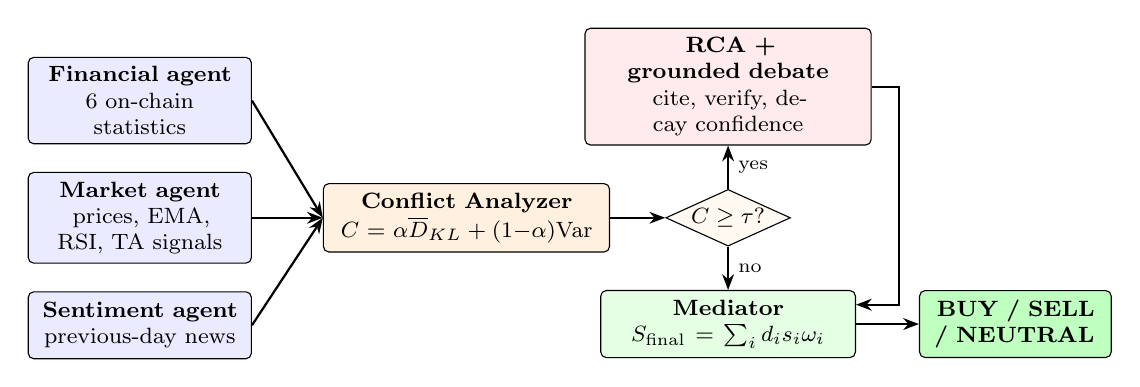
\begin{tikzpicture}[
  node distance=0.35cm and 0.8cm,
  box/.style={draw,rounded corners=2pt,align=center,minimum height=0.85cm,text width=2.6cm,font=\footnotesize,fill=#1},
  box/.default=white,
  arr/.style={-{Stealth[length=2mm]},thick}]
  \node[box=blue!8] (mkt) {\textbf{Market agent}\\prices, EMA, RSI, TA signals};
  \node[box=blue!8,above=of mkt] (fin) {\textbf{Financial agent}\\6 on-chain statistics};
  \node[box=blue!8,below=of mkt] (sen) {\textbf{Sentiment agent}\\previous-day news};
  \node[box=orange!12,right=0.9cm of mkt,text width=3.4cm] (ca) {\textbf{Conflict Analyzer}\\[1pt]$C=\alpha\overline{D}_{KL}+(1{-}\alpha)\mathrm{Var}$};
  \node[diamond,draw,aspect=2.2,right=0.7cm of ca,font=\footnotesize,inner sep=0.5pt,fill=orange!5] (dec) {$C\geq\tau$?};
  \node[box=red!8,above=0.55cm of dec,text width=3.4cm] (deb) {\textbf{RCA + grounded debate}\\cite, verify, decay confidence};
  \node[box=green!10,below=0.55cm of dec,text width=3.0cm] (med) {\textbf{Mediator}\\$\Sfinal=\sum_i d_i s_i \omega_i$};
  \node[box=green!25,right=0.8cm of med,text width=2.2cm] (out) {\textbf{BUY / SELL / NEUTRAL}};
  \foreach \n in {fin,mkt,sen} \draw[arr] (\n.east) -- (ca.west);
  \draw[arr] (ca) -- (dec);
  \draw[arr] (dec) -- node[right,font=\scriptsize]{yes} (deb);
  \draw[arr] (dec) -- node[right,font=\scriptsize]{no} (med);
  \draw[arr] (deb.east) -- ++(0.35,0) |- ([yshift=7pt]med.east);
  \draw[arr] (med) -- (out);
\end{tikzpicture}
\caption{Conflict-aware multi-agent pipeline. Each source has its own agent; disagreement is measured and, above a
threshold, explained and debated with verified citations before aggregation.}
\label{fig:arch}
\end{figure*}

Figure~\ref{fig:arch} shows the pipeline. For a decision at the open of day $D$, three specialists analyse their own
source; a Conflict Analyzer measures their disagreement; above a threshold it triggers root-cause analysis (RCA) and
debate; a Mediator aggregates the final opinions into a signal.

\subsection{Specialist agents}
The \emph{Market} agent reads the last seven daily opens, EMA20/50 and RSI14 of opens, and the three technical signals
CryptoTrade uses (moving-average crossover, MACD, Bollinger bands). The \emph{Financial} agent reads six on-chain
transaction statistics of day $D{-}1$ with their day-over-day change. The \emph{Sentiment} agent reads the news
articles of day $D{-}1$. Every evidence item (a metric, a news sentence) is placed on its own line so that later stages
can cite it precisely. Each agent returns a signal, a belief $(d_i, s_i)$ with direction $d_i\in\{-1,0,1\}$ and
strength $s_i\in[0,1]$, a reasoning path, and metadata. A noise score $e_i$ is computed from data rather than by the
LLM: $1-|\text{RSI}-50|/50$ for Market, the mean absolute daily change of on-chain metrics divided by 30\% (capped at
1) for Financial, and a neutral 0.5 for Sentiment since the dataset has no fear-and-greed index.

\subsection{Conflict Analyzer}
Each belief is mapped to a distribution over \{down, up\}, $P_i=(0.5-0.5x_i,\,0.5+0.5x_i)$ with $x_i=d_i s_i$, so a
weak opinion stays close to uniform. The conflict score combines the mean pairwise KL divergence~\citep{kullback1951}
over ordered pairs with the variance of the signed beliefs:
\begin{equation}
\begin{aligned}
C={}&\alpha\,\tfrac{1}{N(N-1)}\textstyle\sum_{i\neq j}D_{KL}(P_i\,\|\,P_j)\\
&+(1-\alpha)\,\mathrm{Var}(x_1,\dots,x_N),
\end{aligned}
\end{equation}
with $\alpha=0.6$ and $N=3$. When $C\geq\tau=0.4$, rule-based categories (signal, temporal, reliability, redundancy
conflict) are assigned and an LLM writes an RCA of 1--3 cited claims explaining the disagreement.

\subsection{Grounded debate}
In each of two rounds, agent $i$ receives a rebuttal strength
\begin{equation}
\begin{aligned}
R_i=\mathrm{clip}\Big(&\tfrac{1}{1.5(N-1)}\textstyle\sum_{j\neq i}\big[w_b D_{\cos}\\
&+w_e D_{J}+w_l D_{L}\big],\,0,\,1\Big),
\end{aligned}
\end{equation}
averaging the cosine distance between signed beliefs, the Jaccard distance between evidence vocabularies and the
normalised Levenshtein distance between reasoning paths ($w_b=w_e=w_l=1/3$). Its confidence decays as
$s_i\leftarrow s_i e^{-\beta R_i}$ with $\beta=0.35$, and the agent rewrites its reasoning given the accumulated debate
history (as in MADAM-RAG's aggregator), all agents' evidence and a constraint to stay within its role. The update changes
the \emph{strength} $s_i$ but never the \emph{direction} $d_i$.

\paragraph{Citation verification.}
Every RCA and debate output consists of 1--3 claims labelled fact, inference or hypothesis, each citing an evidence id
and a line id. Code checks the schema and resolves the quoted line itself, so the model never copies numbers. A
separate LLM call then judges each claim as supported, unsupported or contradicted against the full evidence; a failed
or missing review counts as rejection. After one retry, a rejected update is rolled back entirely, including the
confidence decay, so unsupported arguments cannot move the decision. The day is still traded and flagged.

\subsection{Mediator}
Agent weights are $\omega_i=(1-e_i)(1-r_i)\,e^{-\gamma\Delta t_i}$ with redundancy $r_i$ (0.05--0.1), data age
$\Delta t_i$ in seconds and $\gamma=10^{-5}$. The aggregate $\Sfinal=\sum_i d_i s_i\omega_i$ yields BUY if
$\Sfinal>0.05$, SELL if $\Sfinal<-0.05$ and NEUTRAL otherwise. Signals map to actions $+0.5$, $-0.5$ and $0$ (buy with
half the cash, sell half the coins, hold), the sizing CryptoTrade uses for its rule baselines.

% =====================================================================
\section{Experimental Setup}

\paragraph{Data and periods.}
We use CryptoTrade's public BTC dataset: daily prices (CoinMarketCap), six on-chain statistics (Dune) and up to five
filtered news articles per day (Google News). We keep the paper's three test periods: bull (2023-10-01 to 12-01,
61 trading days, BTC +39.7\%), sideways (06-17 to 08-25, 69 days, $-$0.8\%) and bear (04-12 to 06-16, 65 days,
$-$15.6\%).

\paragraph{Baseline reproduction.}
We reimplement CryptoTrade's environment, four prompts, agent loop and rule baselines. The public code differs from
the paper (it disables two of the three technical signals and reflects over three days), so we follow the paper: three
signals and seven-day reflection. Running the original code side by side, our six rule strategies match its returns and
Sharpe ratios exactly on all three periods, and therefore also match the paper's Table~2; the four prompts are
identical over 12 steps for the same action sequence. On our local model, CryptoTrade reaches +30.47\% / $-$1.63\% /
$-$11.72\% versus +26.35\% / $-$4.07\% / $-$11.72\% reported with GPT-4, so the reproduction is faithful and the model is
a capable backbone.

\paragraph{Environment and model.}
Both systems trade in CryptoTrade's environment: \$1M split evenly between cash and BTC, one action in $[-1,1]$ per
day, no shorting, 0.4\% fee plus fixed gas, execution at the open. Both use \texttt{gemma-4-26b-a4b} (4-bit QAT) served
locally by LM Studio on a MacBook M1 Pro, temperature 0, with all calls cached for exact reruns. At the open of $D$ both
systems see prices up to that open and on-chain data and news of $D{-}1$; a unit test confirms the inputs coincide with
CryptoTrade's on all 61 bull days.

\paragraph{Configurations and metrics.}
We compare CryptoTrade \emph{full} (all sources and reflection), CryptoTrade \emph{market-only} (technical signals
only), our full system, and ablations derived offline from the same run by re-aggregating saved opinions: without
debate, Market only, Market+Financial and Market+Sentiment. We report total return, Sharpe ratio~\citep{sharpe1966}
(mean over standard deviation of daily returns, as in CryptoTrade) and directional accuracy, the share of trading days
whose direction matches the open-to-open move.

% =====================================================================
\section{Results}

\begin{table}[t]
\centering
\small
\setlength{\tabcolsep}{3.5pt}
\resizebox{\columnwidth}{!}{%
\begin{tabular}{lrrrr}
\toprule
Method & Bull & Side & Bear & Avg \\
\midrule
Buy \& Hold & 39.66 & $-$0.83 & $-$15.61 & 7.74 \\
SLMA (rule) & 38.53 & $-$3.14 & $-$7.68 & 9.24 \\
\midrule
CryptoTrade full & 30.47 & $-$1.63 & $-$11.72 & \textbf{5.71} \\
CryptoTrade market-only & $-$3.31 & 1.76 & $-$8.49 & $-$3.35 \\
\midrule
Ours full & 16.14 & 1.62 & $-$16.63 & 0.38 \\
\quad w/o debate & 13.53 & 1.60 & $-$18.36 & $-$1.08 \\
\quad Market + Sentiment & 12.00 & 2.57 & $-$12.55 & 0.67 \\
\quad Market + Financial & 2.12 & \textbf{6.51} & $-$18.62 & $-$3.33 \\
\quad Market only & 3.09 & 2.61 & $-$10.01 & $-$1.44 \\
\bottomrule
\end{tabular}}
\caption{Total return (\%) on the three BTC periods with the same local LLM.}
\label{tab:main}
\end{table}

\subsection{RQ1: explicit versus implicit conflict handling}
Table~\ref{tab:main} shows that our full system averages +0.38\%, above CryptoTrade market-only ($-$3.35\%) but below
CryptoTrade full (+5.71\%) and Buy \& Hold (+7.74\%). It wins only in the sideways period. The gap is not explained by
prediction quality: in the bull period the two systems have almost the same directional accuracy (55.3\% vs.\ 55.1\%),
yet our return is about half. CryptoTrade chooses its own position size and typically commits 0.8--1.0 of its cash when
confident, while our system trades a fixed half; with no shorting, every SELL in a rally forfeits gains that cannot be
recovered. Explicit conflict handling, in its current form, does not beat implicit fusion.

\subsection{RQ2: source value is regime-dependent}

\begin{table}[t]
\centering
\small
\begin{tabular}{lrrr}
\toprule
Added to Market only & Bull & Side & Bear \\
\midrule
+ Sentiment (news) & +8.9 & $-$0.0 & $-$2.5 \\
+ Financial (on-chain) & $-$1.0 & +3.9 & $-$8.6 \\
+ both, with debate & +13.1 & $-$1.0 & $-$6.6 \\
\bottomrule
\end{tabular}
\caption{Return change (percentage points) from adding sources to the Market-only configuration.}
\label{tab:sources}
\end{table}

Table~\ref{tab:sources} isolates each source. News helps strongly in the bull period and slightly hurts in the bear
period. On-chain data helps in the sideways period, where Market+Financial reaches the best directional accuracy of all
configurations (63.0\%), but costs 8.6 points in the bear period. In the bear period, Market only is our best
configuration: every added source makes losses worse. The extra sources carry signal, but its sign depends on the regime,
and a fixed-weight aggregator cannot exploit it.

\subsection{RQ3: debate reduces conflict but rarely resolves it}

\begin{table}[t]
\centering
\small
\setlength{\tabcolsep}{3pt}
\resizebox{\columnwidth}{!}{%
\begin{tabular}{lccc}
\toprule
 & Bull & Side & Bear \\
\midrule
Debate days & 36/61 & 32/69 & 31/65 \\
Conflict before $\rightarrow$ after & .63$\rightarrow$.24 & .61$\rightarrow$.22 & .60$\rightarrow$.22 \\
Flagged (rejected update) & 10 & 6 & 8 \\
Return gain vs.\ no debate & +2.6 & +0.0 & +1.7 \\
Final BUY / SELL / NEUTRAL & 19/28/14 & 27/23/19 & 26/24/15 \\
\bottomrule
\end{tabular}}
\caption{Debate statistics and final signal distribution of our full system.}
\label{tab:debate}
\end{table}

Debate fires on 99 of 195 days (Table~\ref{tab:debate}) and cuts the mean conflict score from about 0.61 to 0.22. It
never hurts returns. Yet it changes the final signal on only 11 days, always from BUY or SELL to NEUTRAL, and on none of
them does a wrong call become right or vice versa: the gain comes from staying out on uncertain days. The cause is by
design: debate decays the strength of contested opinions but never flips their direction, so opposing beliefs shrink
towards zero together. The conflict score falls because the agents become less certain, not because they agree.
Debate thus acts as a risk filter rather than an error-correction mechanism, a distinction that a lower conflict score
alone would hide.

\subsection{Analysis: hidden aggregation bias and trend blindness}
Two further observations explain the weak bear-period results. First, the time-decay penalty treats day-old data as
stale: on-chain data and news are from $D{-}1$, so their factor is $e^{-0.864}\approx0.42$ against 1 for prices. With
equal noise, the Market agent therefore carries about 2.5 times the weight of each other agent, and Sentiment's weight
is fixed near $0.5\times0.9\times0.42\approx0.19$. A design choice intended for live freshness becomes a structural bias
in a daily backtest. Second, signals do not follow the trend: during a 40\% rally the system issued 28 SELLs against 19
BUYs, and during the decline 26 BUYs against 24 SELLs, consistent with agents reacting to short-term RSI and daily news.

\paragraph{Cost.} Per period, CryptoTrade full needs about 50 minutes and our system about 4.6 hours on the laptop,
because of the RCA, debate and verification calls; the monetary cost of both is zero with a local model.

% =====================================================================
\section{Conclusion}
Under identical data, environment and model, separating sources into specialised agents and handling their conflict
explicitly does not yet outperform CryptoTrade's implicit fusion, even though directional accuracy is on par. The
study yields three lessons for conflict-aware agent design: the value of a source is regime-dependent and can change
sign; a debate that only decays confidence lowers measured disagreement without resolving it; and aggregation
penalties can encode unintended biases that dominate the outcome. Our next step is a trend detector computed from past
prices that both re-weights agents by regime and filters counter-trend signals, tuned on unused dates of the dataset
before evaluation on the test periods; allowing well-supported direction changes during debate and confidence-based
position sizing are natural extensions.

\section*{Limitations}
Each period has only 61--69 trading days, so differences of a few points are not statistically significant. We study
one asset and one 26B-parameter model; results may differ for ETH, SOL or larger models. The model may have seen 2023
market data during pretraining; this affects both systems equally but may inflate absolute returns. The $\pm0.5$
action mapping and the parameters of the conflict score, debate and Mediator were set by design intuition and not
tuned. Ablations are re-aggregations of one run rather than independent runs.

\section*{Ethics Statement}
This work studies trading signals in simulation and does not constitute financial advice. The CryptoTrade dataset is used
under its CC BY-NC-SA 4.0 licence for non-commercial research.

\bibliography{references}

\appendix
\section{Parameters}
\label{app:params}
Conflict Analyzer: $\alpha=0.6$, $\tau=0.4$, no-conflict ceiling 0.15. Debate: 2 rounds, $\beta=0.35$, equal rebuttal
weights. Mediator: $\gamma=10^{-5}$\,s$^{-1}$, signal band 0.05, redundancy 0.05 (Market) and 0.1 (Financial,
Sentiment). Action mapping BUY/SELL/NEUTRAL $=+0.5/-0.5/0$.

\section{Directional accuracy and trading days}
\begin{table}[h]
\centering
\small
\setlength{\tabcolsep}{3pt}
\begin{tabular}{lccc}
\toprule
Method & Bull & Side & Bear \\
\midrule
CryptoTrade full & 55.1 / 49 & 45.6 / 68 & 50.0 / 56 \\
CryptoTrade mkt-only & 48.1 / 52 & 45.2 / 62 & 56.9 / 58 \\
Ours full & 55.3 / 47 & 56.0 / 50 & 48.0 / 50 \\
\quad w/o debate & 55.8 / 52 & 54.7 / 53 & 45.3 / 53 \\
\quad Market + Sent. & 52.9 / 51 & 51.1 / 47 & 49.0 / 51 \\
\quad Market + Fin. & 58.3 / 48 & 63.0 / 54 & 45.8 / 48 \\
\quad Market only & 54.5 / 44 & 54.8 / 42 & 50.0 / 40 \\
\bottomrule
\end{tabular}
\caption{Directional accuracy (\%) / number of trading (non-NEUTRAL) days.}
\end{table}

\end{document}
